% !TeX program = xelatex
\documentclass[a4paper,10pt]{article}

% ============================================================================
% សន្លឹកកិច្ចការសិស្សបំពេញចន្លោះ ស-ខ្មៅ និងប្លង់ក្ដារខៀន/ចម្លើយគ្រូ (គ្មាន LCD / គ្មានកន្ត្រៃ)
% មេរៀនទី៥ (៣.១)៖ ពន្លាតការេនៃទ្វេធា និង (a-b)(a+b) — ត្រូវគ្នានឹង LS_Plan_ALG55.tex
% ============================================================================
\usepackage[a4paper, left=1.0cm, right=1.0cm, top=0.75cm, bottom=1.00cm, footskip=0.52cm]{geometry}
\usepackage{amsmath}
\usepackage{unicode-math}
\usepackage{fontspec}
\usepackage{array, colortbl}
\usepackage[table]{xcolor}
\usepackage{enumitem}
\usepackage{pifont}
\usepackage{fancyhdr}
\usepackage{lastpage}
\usepackage{tikz}
\usepackage[most]{tcolorbox}
\usetikzlibrary{calc, arrows.meta, decorations.pathreplacing, positioning, babel}

\makeatletter
\let\@expl@@@mark@update@singlecol@structures@@\relax
\makeatother

\providecommand{\NGSFindFonts}{%
  \IfFileExists{C:/Windows/Fonts/cambria.ttc}{%
    \def\NGSSysPath{C:/Windows/Fonts/}%
    \def\NGSUserPath{C:/Users/KIT/AppData/Local/Microsoft/Windows/Fonts/}%
  }{%
    \IfFileExists{./fonts/KhmerOSsiemreap.ttf}{\def\NGSSysPath{./fonts/}\def\NGSUserPath{./fonts/}}{%
    \IfFileExists{../fonts/KhmerOSsiemreap.ttf}{\def\NGSSysPath{../fonts/}\def\NGSUserPath{../fonts/}}{%
    \IfFileExists{../../fonts/KhmerOSsiemreap.ttf}{\def\NGSSysPath{../../fonts/}\def\NGSUserPath{../../fonts/}}{%
    \IfFileExists{../../../fonts/KhmerOSsiemreap.ttf}{\def\NGSSysPath{../../../fonts/}\def\NGSUserPath{../../../fonts/}}{%
    \IfFileExists{../../../../fonts/KhmerOSsiemreap.ttf}{\def\NGSSysPath{../../../../fonts/}\def\NGSUserPath{../../../../fonts/}}{%
    \IfFileExists{../../../../../fonts/KhmerOSsiemreap.ttf}{\def\NGSSysPath{../../../../../fonts/}\def\NGSUserPath{../../../../../fonts/}}{%
    \IfFileExists{../../../../../../fonts/KhmerOSsiemreap.ttf}{\def\NGSSysPath{../../../../../../fonts/}\def\NGSUserPath{../../../../../../fonts/}}{%
      \def\NGSSysPath{../../../../../../../fonts/}\def\NGSUserPath{../../../../../../../fonts/}%
    }}}}}}}%
  }%
}
\NGSFindFonts

\setmathfont[Path={\NGSSysPath}, FontIndex=1, Scale=1.02]{cambria.ttc}
\defaultfontfeatures{Ligatures=TeX}

\setmainfont[
  Path={\NGSUserPath}, Extension=.ttf, Script=Khmer,
  BoldFont={KhmerOSsiemreap}, BoldFeatures={FakeBold=1.8},
  ItalicFont={KhmerOSsiemreap}, ItalicFeatures={FakeSlant=0.25},
  BoldItalicFont={KhmerOSsiemreap}, BoldItalicFeatures={FakeBold=1.8, FakeSlant=0.25}
]{KhmerOSsiemreap}

\newfontfamily\muol[Path={\NGSUserPath}, Extension=.ttf, Script=Khmer]{KhmerOSmuollight}
\newfontfamily\TimesEn[Path={\NGSSysPath}, Extension=.ttf, BoldFont={timesbd}, ItalicFont={timesi}, BoldItalicFont={timesbi}]{times}
\newfontfamily\CalibriFont[Path={\NGSSysPath}, Extension=.ttf]{calibri}

\XeTeXlinebreaklocale "km"
\XeTeXlinebreakskip = 0pt plus 1pt minus 0.1pt

\definecolor{panelgray}{gray}{0.94}
\definecolor{headgray}{gray}{0.85}

\pagestyle{fancy}
\fancyhf{}
\renewcommand{\headrulewidth}{0pt}
\fancyfoot[L]{\fontsize{7.4pt}{9.5pt}\selectfont អនុវិទ្យាល័យព្រះក្រសាំង \en{|} គ្រូ៖ ហុក ប៊ុនថែន \en{|} មេរៀនទី៥ (៣.១) សមភាពសំខាន់ៗការេទ្វេធា \en{|} ថ្ងៃពុធ ទី៩ ខែធ្នូ ឆ្នាំ២០២៦}
\fancyfoot[R]{\fontsize{7.8pt}{10pt}\selectfont ទំព័រ \en{\thepage\ / \pageref{LastPage}}}

\setlength{\parindent}{0pt}
\setlength{\parskip}{0pt}
\setlength{\tabcolsep}{4pt}

\newcommand{\en}[1]{{\TimesEn #1}}
\newcommand{\enbf}[1]{{\TimesEn\bfseries #1}}
\newcommand{\unit}[1]{\,\text{\en{#1}}}
\newcommand{\riel}{\,\text{៛}}
\newcommand{\cnum}[1]{\mbox{\fontsize{10pt}{12pt}\selectfont\ding{\numexpr181+#1\relax}}}
\newcommand{\chkbox}{\tikz[baseline=-0.15ex]\draw[black, line width=0.85pt, fill=white] (0,0) rectangle (0.24cm,0.24cm);}
\newcommand{\ansbox}[1][2.0cm]{\,\tikz[baseline=-0.65ex]\draw[black, line width=0.65pt, fill=white] (0,0) rectangle (#1, 0.42cm);\,}
\newcommand{\dotline}[1][2.2cm]{\makebox[#1]{\dotfill}}

\newcommand{\pagebanner}[2]{%
  \begin{tcolorbox}[
    enhanced, sharp corners, colback=headgray, colframe=black,
    boxrule=1.05pt, boxsep=1pt, top=2.5pt, bottom=2.5pt, left=6pt, right=6pt,
    after skip=3.5pt
  ]
    {\muol\fontsize{9.0pt}{13.2pt}\selectfont #1}\hfill{\fontsize{8.0pt}{11.2pt}\selectfont\textbf{#2}}
  \end{tcolorbox}%
}

\newcommand{\secstrip}[2]{%
  \vspace{3pt}%
  \begin{tcolorbox}[
    enhanced, sharp corners, colback=panelgray, colframe=black,
    boxrule=0.8pt, boxsep=0.8pt, top=2pt, bottom=2pt, left=5pt, right=5pt,
    after skip=3pt
  ]
    {\muol\fontsize{8.5pt}{12.2pt}\selectfont #1}\hfill{\fontsize{7.8pt}{10.8pt}\selectfont\textit{#2}}
  \end{tcolorbox}%
}

\newcolumntype{L}[1]{>{\raggedright\arraybackslash}p{#1}}
\newcolumntype{C}[1]{>{\centering\arraybackslash}p{#1}}

\begin{document}
\fontsize{9.5pt}{14.5pt}\selectfont

% ============================================================================
% ទំព័រទី ១៖ សន្លឹកកិច្ចការសិស្ស (ផ្នែកមុខ៖ E1 -> E2 -> E3)
% ============================================================================
\pagebanner{សន្លឹកកិច្ចការសិស្ស \enbf{(}៥\enbf{.}៣\enbf{.}១ សមភាពសំខាន់ៗ៖ ការេនៃទ្វេធា និង $(a-b)(a+b)$\enbf{)} \enbf{--} ផ្នែកមុខ}{ថ្នាក់ទី៨ \en{|} សៀវភៅគោល ទំ.៦៣--៦៦}

\begin{tcolorbox}[
  enhanced, sharp corners, colback=white, colframe=black,
  boxrule=0.8pt, boxsep=1.5pt, top=3.5pt, bottom=3.5pt, left=5pt, right=5pt,
  after skip=4pt
]
  \fontsize{9.0pt}{13.0pt}\selectfont
  \textbf{ឈ្មោះសិស្ស៖} \dotline[4.3cm] \quad
  \textbf{សមាជិកក្រុម៖} \dotline[4.3cm] \quad
  \textbf{ថ្នាក់ទី៖} ៨\dotline[0.9cm] \quad
  \textbf{ក្រុមទី៖} \dotline[1.0cm]
\end{tcolorbox}

% --- E1 Engage ---
\secstrip{ផ្នែកទី ១ \enbf{(E1 - Engage)} ៖ បេសកកម្មអន្ទាក់ការេនៃផលបូក $(x + 3)^2$}{រយៈពេល ៣ នាទី (គូស \ding{51} ក្នុង \chkbox)}

\begin{tcolorbox}[
  enhanced, sharp corners, colback=white, colframe=black,
  boxrule=0.8pt, boxsep=2.5pt, top=4pt, bottom=4pt, left=6pt, right=6pt
]
  គេចង់ពន្លាត $(x + 3)^2$ (ទំ.៦៣) ។ សាកជំនួស $x = 2$ បាន $(2 + 3)^2 = 5^2 = \mathbf{25}$ ។ តើសិស្សរូបណាពន្លាតបានត្រឹមត្រូវ?\\[3pt]
  \chkbox\ \textbf{សិស្ស ក៖} $(x + 3)^2 = x^2 + 3^2 = x^2 + 9$ \qquad\qquad
  \chkbox\ \textbf{សិស្ស ខ៖} $(x + 3)^2 = (x + 3)(x + 3) = x^2 + 6x + 9$\\[3pt]
  $\bullet$ \textbf{តេស្តដោយ $x = 2$៖} កន្សោមសិស្ស ក ស្មើ $2^2 + 9 =$ \dotline[1.4cm]; \ ឯកន្សោមសិស្ស ខ ស្មើ $2^2 + 6(2) + 9 =$ \dotline[1.4cm] ។
\end{tcolorbox}

\vspace{3pt}

% --- E2 Explore ---
\secstrip{ផ្នែកទី ២ \enbf{(E2 - Explore)} ៖ សមភាពសំខាន់ៗទាំង ៣ តាមគំរូផ្ទៃក្រឡា និងការពន្លាត (ទំ.៦៣--៦៦)}{រយៈពេល ១១ នាទី}

\textbf{សកម្មភាព ១ (\en{E2-A} — ៦ នាទី)៖ ការេនៃផលបូក $(a+b)^2$ និងការេនៃផលដក $(a-b)^2$ (ទំ.៦៣--៦៤)}

\begin{tcolorbox}[
  enhanced, sharp corners, colback=white, colframe=black,
  boxrule=0.8pt, boxsep=2.5pt, top=4pt, bottom=4pt, left=6pt, right=6pt
]
  \begin{minipage}[c]{3.8cm}
    \centering
    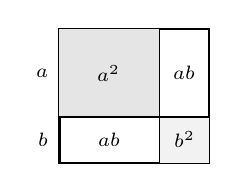
\begin{tikzpicture}[x=1cm, y=1cm, every node/.style={font=\scriptsize, text=black}]
      \draw[black, line width=0.9pt] (0.45,0.10) rectangle (2.35,1.80);
      \fill[gray!20] (0.45,0.68) rectangle (1.72,1.80);
      \fill[gray!10] (1.72,0.10) rectangle (2.35,0.68);
      \draw[black, line width=0.65pt] (1.72,0.10) -- (1.72,1.80);
      \draw[black, line width=0.65pt] (0.45,0.68) -- (2.35,0.68);
      \node at (0.24,1.24) {$a$};
      \node at (0.24,0.39) {$b$};
      \node at (1.08,1.24) {$a^2$};
      \node at (2.04,1.24) {$ab$};
      \node at (1.08,0.39) {$ab$};
      \node at (2.04,0.39) {$b^2$};
    \end{tikzpicture}
  \end{minipage}\hfill
  \begin{minipage}[c]{14.2cm}
    $\bullet$ \textbf{១) ផ្ទៃការេជ្រុង $a+b$ (ទំ.៦៣)៖} បូកផ្ទៃទាំង ៤ ផ្នែក៖ $(a + b)^2 = a^2 + ab + ab + b^2 =$ \ansbox[3.8cm]\\[3pt]
    $\bullet$ \textbf{២) ការេនៃផលដក (ទំ.៦៤)៖} $(a - b)^2 = (a - b)(a - b) = a^2 - ab - ba + (-b)^2 =$ \ansbox[3.8cm]\\[3pt]
    $\bullet$ \textbf{៣) អនុវត្តភ្លាម៖} $(x - 1)^2 = x^2 - 2(x)(1) + 1^2 =$ \dotline[3.4cm] ។
  \end{minipage}
\end{tcolorbox}

\vspace{4pt}
\textbf{សកម្មភាព ២ (\en{E2-B} — ៥ នាទី)៖ ផលគុណ $(a-b)(a+b)$ និងកំសាន្តគណិតវិទ្យា (ទំ.៦៥--៦៦)}

\begin{tcolorbox}[
  enhanced, sharp corners, colback=white, colframe=black,
  boxrule=0.8pt, boxsep=2.5pt, top=4pt, bottom=4pt, left=6pt, right=6pt
]
  $\bullet$ \textbf{១) ពន្លាត $(a - b)(a + b)$ (ទំ.៦៥)៖} $(a - b)(a + b) = a^2 + ab - ba - b^2 =$ \ansbox[2.8cm] ; \quad ឧ. $(x - 2)(x + 2) =$ \dotline[2.4cm]\\[4pt]
  $\bullet$ \textbf{២) កំសាន្តគណិតវិទ្យា (ទំ.៦៦)៖} $(2+1)(2-1)=3, \ (3+2)(3-2)=5 \implies (4+3)(4-3) =$ \dotline[1.2cm], \ $(10+9)(10-9) =$ \dotline[1.2cm]
\end{tcolorbox}

\vfill

% --- E3 Explain ---
\secstrip{ផ្នែកទី ៣ \enbf{(E3 - Explain)} ៖ រូបមន្តសមភាពសំខាន់ៗទាំង ៣ និងធនាគារហេតុផល \enbf{B\&W}}{រយៈពេល ៦ នាទី}

\begin{tcolorbox}[
  enhanced, sharp corners, colback=white, colframe=black,
  boxrule=0.85pt, boxsep=2.5pt, top=4pt, bottom=4pt, left=6pt, right=6pt
]
  $\bullet$ \textbf{(1) ការេនៃផលបូក៖} $(a + b)^2 =$ \ansbox[3.8cm] \qquad
  \textbf{(2) ការេនៃផលដក៖} $(a - b)^2 =$ \ansbox[3.8cm]\\[4pt]
  $\bullet$ \textbf{(3) ផលគុណនៃផលដកនិងផលបូកពីរចំនួន៖} $(a - b)(a + b) =$ \ansbox[3.2cm]\\[4pt]
  \tikz\draw[black, dashed, line width=0.5pt] (0,0) -- (18.4cm,0);\\[3pt]
  \fontsize{8.8pt}{13.0pt}\selectfont
  \textbf{ធនាគារហេតុផល (\en{Warrant Bank})៖} \quad
  \cnum{1} ការេទ្វេធា $(a\pm b)^2$ មាន $3$ តួ (ហាមភ្លេច $\pm 2ab$) \quad
  \cnum{2} តួចុងក្រោយ $(-b)^2 = +b^2$ វិជ្ជមានជានិច្ច\\
  \cnum{3} លើកមេគុណជាការេទាំងមូល $(2m)^2 = 4m^2$ \quad
  \cnum{4} $(a-b)(a+b) = a^2 - b^2$ ស៊ីសងតួកណ្ដាល $+ab - ab = 0$
\end{tcolorbox}

% ============================================================================
% ទំព័រទី ២៖ សន្លឹកកិច្ចការសិស្ស (ផ្នែកខាងខ្នង៖ E4 -> E5 -> កិច្ចការផ្ទះ)
% ============================================================================
\clearpage
\pagebanner{សន្លឹកកិច្ចការសិស្ស \enbf{(}៥\enbf{.}៣\enbf{.}១ ការេនៃទ្វេធា និង $(a-b)(a+b)$\enbf{)} \enbf{--} ផ្នែកខាងខ្នង}{ថ្នាក់ទី៨ \en{|} ទំ.៦៤--៦៦, ៧៣}

% --- E4 Elaborate ---
\secstrip{ផ្នែកទី ៤ \enbf{(E4 - Elaborate)} ៖ លំហាត់គំរូមេគុណទ្វេធា និងមុធាគណនាលេខរហ័ស (ទំ.៦៤--៦៥)}{រយៈពេល ១០ នាទី}

\begin{tcolorbox}[
  enhanced, sharp corners, colback=white, colframe=black,
  boxrule=0.8pt, boxsep=2.5pt, top=4pt, bottom=4pt, left=6pt, right=6pt
]
  \textbf{១) ពន្លាតកន្សោមដែលមានមេគុណ និងប្រភាគ (លំហាត់គំរូ ទំ.៦៤--៦៥)៖}\\[3pt]
  \hspace*{0.3cm}$\bullet$ $(2m + 3n)^2 = (2m)^2 + 2(2m)(3n) + (3n)^2 =$ \ansbox[4.8cm]\\[3pt]
  \hspace*{0.3cm}$\bullet$ $\left(\dfrac{1}{2}m - n\right)^2 =$ \ansbox[4.2cm] \qquad
  $\bullet$ $\left(\dfrac{1}{2}m - 3n\right)\left(\dfrac{1}{2}m + 3n\right) =$ \ansbox[3.4cm]\\[5pt]
  \textbf{២) មុធាគណនារហ័សដោយប្រើសមភាពសំខាន់ៗ (ទំ.៦៤--៦៥)៖}\\[3pt]
  \hspace*{0.3cm}$\bullet$ $101^2 = (100 + 1)^2 = 100^2 + 200 + 1 =$ \ansbox[2.4cm] \qquad
  $\bullet$ $99^2 = (100 - 1)^2 = 100^2 - 200 + 1 =$ \ansbox[2.4cm]\\[3pt]
  \hspace*{0.3cm}$\bullet$ $101 \times 99 = (100 + 1)(100 - 1) = 100^2 - 1^2 =$ \ansbox[2.6cm]\\[3pt]
  \fontsize{8.8pt}{13.0pt}\selectfont
  \textbf{ឆ្លុះបញ្ចាំង (\en{EIA Looking-Back})៖} ហេតុអ្វី $(a - b)^2$ ស្មើនឹង $(b - a)^2$? \textbf{ព្រោះ} \dotline[5.5cm] ។
\end{tcolorbox}

\vspace{4pt}

% --- E5 Evaluate ---
\secstrip{ផ្នែកទី ៥ \enbf{(E5 - Evaluate)} ៖ ប្រតិបត្តិ (ទំ.៦៤--៦៥) សំណួរវិនិច្ឆ័យ \enbf{A--D} និងសំបុត្រចេញ}{រយៈពេល ១០ នាទី}

\begin{tcolorbox}[
  enhanced, sharp corners, colback=white, colframe=black,
  boxrule=0.8pt, boxsep=2.5pt, top=4pt, bottom=4pt, left=6pt, right=6pt
]
  \textbf{១) ប្រតិបត្តិជាក្រុម (ទំ.៦៤ និង ទំ.៦៥)៖}\\[3pt]
  \hspace*{0.3cm}$\bullet$ ទំ.៦៤ (ក)៖ $(x + 2)^2 =$ \ansbox[3.8cm] \qquad\qquad
  ទំ.៦៥ (ក)៖ $(x - 5)^2 =$ \ansbox[3.8cm]\\[3pt]
  \hspace*{0.3cm}$\bullet$ ទំ.៦៥ ខាងក្រោម (គ)៖ $(2x + 3y)(2x - 3y) =$ \ansbox[3.8cm]\\[4pt]
  \textbf{២) បិទបេសកកម្ម \en{E1}៖} សិស្ស \dotline[1.0cm] ត្រឹមត្រូវ ព្រោះ $(x + 3)^2 =$ \ansbox[3.8cm] (ខុសពី $x^2 + 9$ ចំនួនតួ $+6x$) ។
\end{tcolorbox}

\vspace{4pt}

\begin{tcolorbox}[
  enhanced, sharp corners, colback=white, colframe=black,
  boxrule=0.8pt, boxsep=2.5pt, top=4pt, bottom=4pt, left=6pt, right=6pt
]
  \textbf{៣) សំណួរវិនិច្ឆ័យ \en{A--D} (ពន្លាតការេនៃទ្វេធា $(3x - 2y)^2$ — គូសរង្វង់ រួចលើកម្រាមដៃ ១--៤)៖}\\[3pt]
  \textbf{\en{A.}} $9x^2 - 4y^2$ \qquad
  \textbf{\en{B.}} $9x^2 - 12xy - 4y^2$ \qquad
  \textbf{\en{C.}} $3x^2 - 12xy + 2y^2$ \qquad
  \textbf{\en{D.}} $9x^2 - 12xy + 4y^2$\\[4pt]
  \tikz\draw[black, dashed, line width=0.5pt] (0,0) -- (18.4cm,0);\\[3pt]
  \textbf{៤) សំបុត្រចេញ ៦០ វិនាទី (ទំ.៧៣ \#9)៖} គណនារហ័ស $39 \times 41 = (40 - 1)(40 + 1) =$ \ansbox[3.2cm] ។
\end{tcolorbox}

\vfill

% --- Homework ---
\begin{tcolorbox}[
  enhanced, sharp corners, colback=panelgray, colframe=black,
  boxrule=0.95pt, boxsep=2pt, top=3.5pt, bottom=3.5pt, left=6pt, right=6pt
]
  {\muol\fontsize{9.0pt}{13.0pt}\selectfont កិច្ចការផ្ទះ \enbf{(}សៀវភៅគោល ទំ.៦៤--៦៥ និង ទំ.៧៣ លេខ ៨, ៩\enbf{)}}\\[2.5pt]
  \fontsize{8.8pt}{13.0pt}\selectfont
  $\bullet$ \textbf{១) ប្រតិបត្តិទំ.៦៤ (ខ, គ) និង ទំ.៦៥ (ខ, ឃ)៖} ពន្លាត $(3a+1)^2$, $(2x+3y)^2$, $(3a-2b)^2$ និង $\left(\dfrac{1}{5}t - u\right)\left(\dfrac{1}{5}t + u\right)$ ។\\
  $\bullet$ \textbf{២) ទំ.៧៣ \#8 ក, ខ និង \#9៖} ស្រាយបញ្ជាក់ $(1+x)(1-x)(1+x^2)=1-x^4$, $5b^2+3(b+1)(b-1)=2b^2+3$; និងគណនា $54\times 66$, $102^2 - 101^2$ ។
\end{tcolorbox}

% ============================================================================
% ទំព័រទី ៣៖ ទំព័រគ្រូបង្រៀន (គំរូប្លង់ក្ដារខៀន ៣ ផ្នែក + ចម្លើយផ្ទៀងផ្ទាត់រហ័ស)
% ============================================================================
\clearpage
\pagebanner{ទំព័រគ្រូបង្រៀន ៖ ប្លង់ក្ដារខៀន \enbf{(}គ្មាន \enbf{LCD)} និងចម្លើយផ្ទៀងផ្ទាត់រហ័ស}{៥.៣.១ ការេនៃទ្វេធា និង $(a-b)(a+b)$ (\en{ALG55})}

\secstrip{១. គំរូប្លង់បែងចែកក្ដារខៀន ៣ ផ្នែក សម្រាប់ថ្នាក់រៀនគ្មាន \enbf{LCD}}{សម្រាប់គ្រូប្រើដីស/ហ្វឺត}

\begin{center}
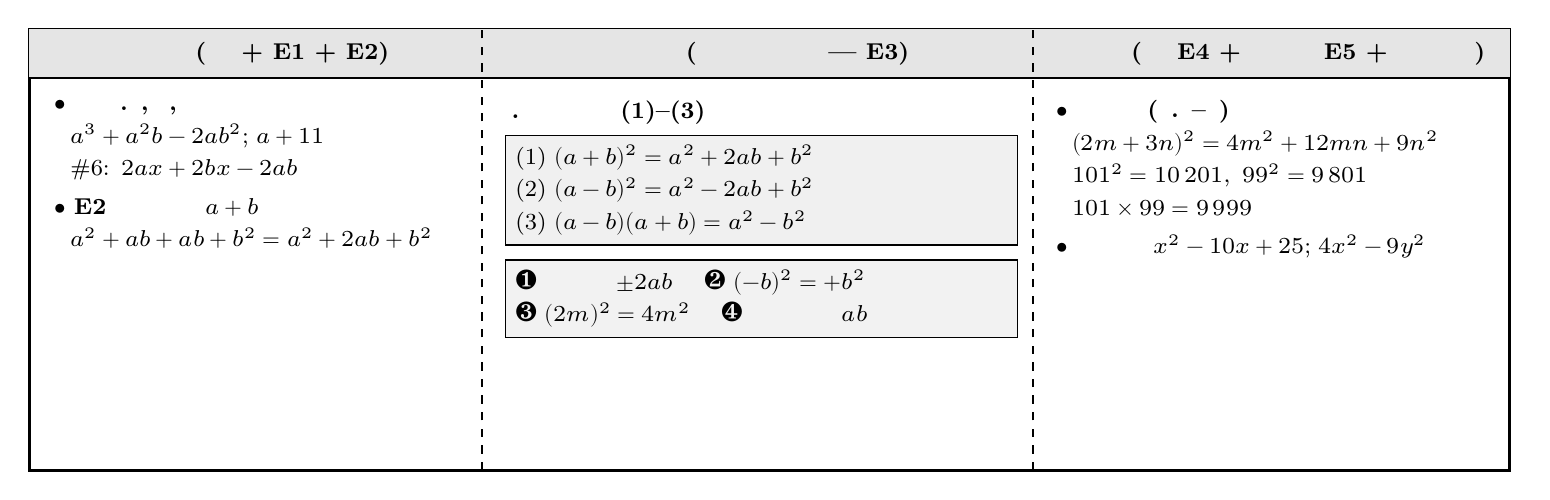
\begin{tikzpicture}[x=1cm, y=1cm, every node/.style={font=\fontsize{8.3pt}{11.8pt}\selectfont, text=black}]
  \draw[black, line width=1.1pt] (0,0) rectangle (18.8,5.60);
  \fill[gray!20] (0,4.98) rectangle (18.8,5.60);
  \draw[black, line width=0.7pt] (0,4.98) -- (18.8,4.98);
  \draw[black, dashed, line width=0.7pt] (5.75,0) -- (5.75,5.60);
  \draw[black, dashed, line width=0.7pt] (12.75,0) -- (12.75,5.60);

  \node at (2.875,5.29) {\textbf{ផ្នែកឆ្វេង (កំណែ + \en{E1} + \en{E2})}};
  \node at (9.25,5.29) {\textbf{ផ្នែកកណ្ដាល (ខ្លឹមសារគោលរក្សាទុក — \en{E3})}};
  \node at (15.775,5.29) {\textbf{ផ្នែកស្ដាំ (គំរូ \en{E4} + ប្រតិបត្តិ \en{E5} + កិច្ចការផ្ទះ)}};

  % Left
  \node[anchor=north west, text width=5.35cm] at (0.20,4.82) {%
    $\bullet$ \textbf{កំណែ ទំ.៦០, ៦២, ៧៣៖}\\
    \hspace*{0.2cm}$a^3+a^2b-2ab^2$; $a+11$\\
    \hspace*{0.2cm}\#6: $2ax+2bx-2ab$\\[2pt]
    $\bullet$ \textbf{\en{E2} គំរូការេជ្រុង $a+b$៖}\\
    \hspace*{0.2cm}$a^2 + ab + ab + b^2 = a^2+2ab+b^2$
  };

  % Center
  \node[anchor=north west, text width=6.65cm] at (5.92,4.82) {%
    {\muol\fontsize{8.5pt}{12pt}\selectfont ៣\enbf{.}១ សមភាពសំខាន់ៗ \enbf{(1)--(3)}}\\[3pt]
    \tikz\node[draw=black, fill=gray!12, inner sep=3.5pt, text width=6.25cm]{%
      (1) $(a + b)^2 = a^2 + 2ab + b^2$\\
      (2) $(a - b)^2 = a^2 - 2ab + b^2$\\
      (3) $(a - b)(a + b) = a^2 - b^2$
    };\\[4pt]
    \tikz\node[draw=black, fill=gray!10, inner sep=3.5pt, text width=6.25cm]{%
      \cnum{1} ហាមភ្លេចតួ $\pm 2ab$ \quad \cnum{2} $(-b)^2 = +b^2$\\
      \cnum{3} $(2m)^2 = 4m^2$ \quad \cnum{4} ឆ្លាស់គ្មានតួ $ab$
    };
  };

  % Right
  \node[anchor=north west, text width=5.8cm] at (12.92,4.82) {%
    $\bullet$ \textbf{លំហាត់គំរូ (ទំ.៦៤--៦៥)៖}\\
    \hspace*{0.2cm}$(2m+3n)^2 = 4m^2+12mn+9n^2$\\
    \hspace*{0.2cm}$101^2 = 10\,201, \ 99^2 = 9\,801$\\
    \hspace*{0.2cm}$101\times 99 = 9\,999$\\[2pt]
    $\bullet$ \textbf{ប្រតិបត្តិ៖} $x^2-10x+25$; $4x^2-9y^2$
  };
\end{tikzpicture}
\end{center}

\vspace{4pt}
\secstrip{២. ចម្លើយផ្ទៀងផ្ទាត់រហ័សសម្រាប់សន្លឹកកិច្ចការសិស្ស \enbf{(}ទំព័រ ១ និង ទំព័រ ២\enbf{)}}{\en{Answer Key}}

\begin{tcolorbox}[
  enhanced, sharp corners, colback=white, colframe=black,
  boxrule=0.8pt, boxsep=2pt, top=4pt, bottom=4pt, left=6pt, right=6pt
]
  \fontsize{9.0pt}{13.5pt}\selectfont
  $\bullet$ \textbf{ផ្នែក \en{E1}៖} \textbf{សិស្ស ខ} ត្រឹមត្រូវ ($x^2+6x+9$) ព្រោះពេល $x=2$ បាន $4+12+9 = 25 = 5^2$ (សិស្ស ក បានត្រឹម $13 \neq 25$) ។\\[2pt]
  $\bullet$ \textbf{ផ្នែក \en{E2}៖} \textbf{សកម្មភាព ១៖} $a^2+2ab+b^2$; $a^2-2ab+b^2$; $x^2-2x+1$ ។ \textbf{សកម្មភាព ២៖} $a^2-b^2$; $x^2-4$; $7$ និង $19$ ។\\[2pt]
  $\bullet$ \textbf{ផ្នែក \en{E4}៖} ១) $4m^2+12mn+9n^2$; $\frac{1}{4}m^2-mn+n^2$; $\frac{1}{4}m^2-9n^2$; ២) $10\,201$; $9\,801$; $9\,999$ ។\\[2pt]
  $\bullet$ \textbf{ផ្នែក \en{E5}៖} ១) $x^2+4x+4$; $x^2-10x+25$; $4x^2-9y^2$; ២) សិស្ស ខ ($x^2+6x+9$); ៣) \textbf{ជម្រើស \en{D}} ($9x^2-12xy+4y^2$); ៤) $1\,599$ ។
\end{tcolorbox}

\vspace{4pt}
\secstrip{៣. ចម្លើយលម្អិតនៃកិច្ចការផ្ទះ \enbf{(}សម្រាប់ផ្ទៀងនៅដើមម៉ោងបន្ទាប់ ៥\enbf{.}៣\enbf{.}២\enbf{)}}{សៀវភៅគោល ទំ.៦៤--៦៥, ៧៣}

\begin{tcolorbox}[
  enhanced, sharp corners, colback=white, colframe=black,
  boxrule=0.8pt, boxsep=2pt, top=4pt, bottom=4pt, left=6pt, right=6pt
]
  \fontsize{8.8pt}{13.2pt}\selectfont
  $\bullet$ \textbf{១) ទំ.៦៤–៦៥៖} $(3a+1)^2 = \mathbf{9a^2+6a+1}$, \ $(2x+3y)^2 = \mathbf{4x^2+12xy+9y^2}$, \ $(3a-2b)^2 = \mathbf{9a^2-12ab+4b^2}$, \ $(\frac{1}{5}t-u)(\frac{1}{5}t+u) = \mathbf{\frac{1}{25}t^2 - u^2}$ ។\\[2pt]
  $\bullet$ \textbf{២) ទំ.៧៣ \#8 ក៖} $(1-x^2)(1+x^2) = \mathbf{1-x^4}$; \ \textbf{ខ៖} $5b^2+3(b^2-1) = 8b^2-3$ \textit{(កត់សម្គាល់៖ បើ $5b^2-3(b+1)(b-1) = 2b^2+3$)}; \ \textbf{\#9៖} $54\times 66 = (60-6)(60+6) = \mathbf{3\,564}$; \ $102^2-101^2 = (102-101)(102+101) = \mathbf{203}$ ។
\end{tcolorbox}

\end{document}
